
\section{File Systems}

\begin{frame}{File Systems - Introducción}
 \begin{itemize}
 \item Aplicaciones de computadoras necesitan almacenar y recuperar información
 \item Tres requerimientos fundamentales para el almacenamiento de la información:
  \begin{itemize}
   \item Posibilidad de almacenar una gran cantidad de información
   \item La información debe permanecer disponible después que finaliza el proceso que 
     la está utilizando
   \item Posibilidad de que los procesos accedan concurrentemente a la información
  \end{itemize}
  \item Información almacenada en archivos (files). Salvo excepciones, la entrada y salida de 
    los procesos es mediante archivos
  \item File System es la parte del SO que se encarga del manejo de los archivos
 \end{itemize}
\end{frame}

\begin{frame}{File Systems - Introducción}
 \begin{block}{Archivo}
   Un archivo es un conjunto de información relacionada almacenada en un dispositivo secundario y
    que tiene un nombre
 \end{block}
 \begin{itemize}  
  \item Tres componentes asociados con un archivo:
  \begin{itemize}
   \item Nombre
   \item Metadata 
   \item Datos 
  \end{itemize} 
 \end{itemize}
 \begin{center}
  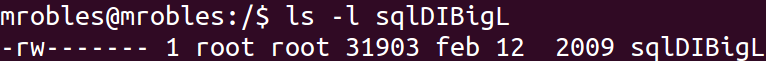
\includegraphics[width=0.9\textwidth]{images/files1.png}
 \end{center} 
\end{frame}

\begin{frame}{File Systems - Introducción}
 \begin{block}{File System}
   Un file system es una abstracción que soporta la creación, borrado, modificación de archivos y de su
   organización en directorios
 \end{block}
 \begin{itemize}
  \item También administra el control de acceso a los archivos y el espacio en disco asignado a él
  \item File systems operan sobre bloques de datos (conjunto consecutivo de sectores)
  \item Archivos son almacenados en una estructura jerárquica de tipo árbol
  \item Define convenciones para el nombrado de archivos
  \item File system usados en discos, CDs, etc.; otros proveen acceso por la red (NFS, SMB, etc.); otros
    son virtuales (procfs)
 \end{itemize}
\end{frame}

\begin{frame}{File Systems - Linux Ext2}
 \begin{itemize}
  \item Primer sector no es administrado por Ext2
  \item Resto del file system dividido en ``block groups''
  \item Block groups reducen la fragmentación y aumenta la velocidad de acceso
  \item ``Superblock'' y ``Group Descriptors Table'' replicado en block groups para backup
  \item Cada bloque contiene su propio ``Group Descriptor''
  \item La tabla de inodos consiste de una serie de bloques consecutivos, cada uno con un 
    número predefinido de inodos. Todos los inodos de igual tamaño: 128 bytes.
 \end{itemize}
\end{frame}

\begin{frame}{File Systems - Linux Ext2}
 \begin{itemize}
  \item Esquema de un file system Ext2
 \end{itemize} 
 \begin{center}
  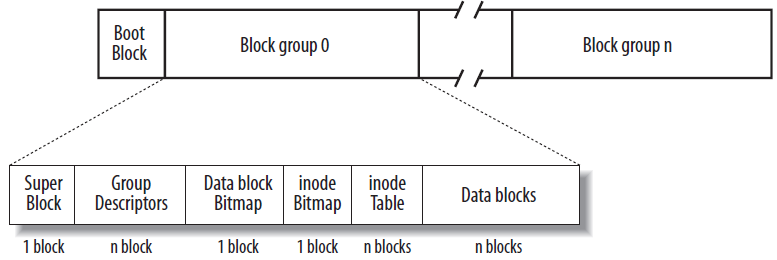
\includegraphics[width=1.0\textwidth]{images/ext2.png}
 \end{center}
\end{frame}

\begin{frame}{File Systems - Linux Ext2 - Inodos}
 \begin{itemize}
  \item Estructura de un inodo:
 \end{itemize} 
 \begin{center}
  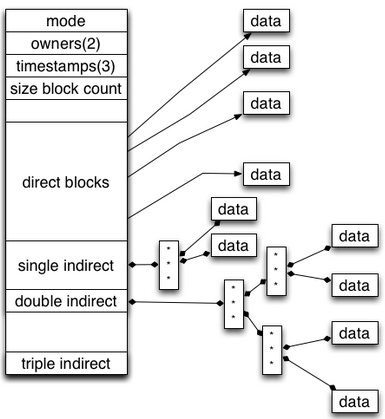
\includegraphics[width=0.5\textwidth]{images/inode1.png}
 \end{center}
\end{frame}

\begin{frame}{File Systems - Particionado}
 \begin{itemize}
  \item Discos pueden ser utilizados completamente por un ``file system'' o pueden ser ``particionado''
  \item Particiones son subdivisiones de un disco entero. SO las presenta como un dispositivo de bloques 
    (como si fuera el disco entero)
  \item Están definidas en un área especial del disco llamado ``partition table''
  \item Cada partición contiene un ``file system'' específico o es una ``raw partitions''
  \item Existen varios tipos de tablas de particiones. Dos más utilizados:
  \begin{itemize}
   \item {\bf Master Boot Record (MBR)}
   \item {\bf Globally Unified Identifier Partition Table (GPT)}
  \end{itemize}
 \end{itemize}
\end{frame}

\begin{frame}{File Systems - MBR}
 \begin{itemize}
  \item MBR se remonta a 1983. PCs basadas en DOS
  \item MBR son los primeros 512 bytes de un dispositivo de almacenamiento (primer sector del
    dispositivo de almancenamiento)
  \item Contiene el ``bootloader'' del sistema operativo y la tabla de particiones
  \item BIOS (Basic Input/Output System) es el encargado de llamar al bootloader
  \item Direccionamiento de hasta 2TB (2,2TB = $2^{32}$ * 512 bytes por sector). 
  \item 4 particiones primarias. Particiones extendidas/lógicas para generar más particiones 
  \item ``Logical Block Addressing(LBA)'' permitió solucionar problemas de direccionamiento 
 \end{itemize}
\end{frame}

\begin{frame}{File Systems - MBR}
 \begin{itemize}
  \item MBR divide los primeros 512 bytes:
  \begin{itemize}
   \item ``Master Boot Code'', también llamado {\it bootloader}, ocupa los primeros 440 bytes
   \item ``Disk signature'': 6 bytes. Identifica el disco al SO.
   \item 16 bytes por cada partición 
   \item ``Signature Word'': 0xAA55
  \end{itemize}
  \item Bootloader encuentra y pasa el control al ``Boot Sector'' de la partición activa
  \item LILO, GRUB, SysLinux son bootloader comunes en Linux
  \item Sectores de 4096KiB permitían hasta 16TiB 
 \end{itemize}
\end{frame}

\begin{frame}{File Systems - MBR}
 \begin{center}
  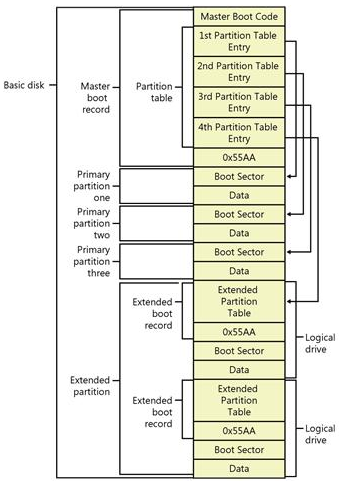
\includegraphics[width=0.43\textwidth]{images/mbr3.png}
 \end{center}
\end{frame}

\begin{frame}{File Systems - GPT}
  \begin{itemize}
   \item Introducida por Intel a finales de los 90 para los Intel Itanium como parte del EFI: 
     ``Extensible Firmware Interface''.
   \item Cedida por Intel al UEFI Forum: ``Unified Extensible Firmware Interface''
   \item No más particiones extendidas/lógicas. 128 particiones por defecto.
   \item LBA de 64 bits $=> 2^{64}$ sectores de 512 bits. Soporta hasta 8ZiB (ó 9,4ZB)
   \item Backup de la GPT final del disco
   \item CRC para proteger el contenido de toda la GPT
   \item Utiliza GUID (``Globally Unique IDentifier'') para referenciar los discos/particiones
  \end{itemize}
\end{frame}

\begin{frame}{File Systems - GPT}
 \begin{itemize}
  \item {\bf Protective MBR:} primer sector del disco (LBA 0, {\it SystemID = 0xEE})
  \item {\bf GUID Partition Table Header:}
  \begin{itemize}
   \item Tamaño mínimo de 16.384 bytes (permiten 128 particiones)
   \item Checksum CRC32 que cubre este sector y toda la tabla de particiones
   \item Ubicación (nro. LBA) de las 2 GPT (original y backup). Tambén indica su tamaño 
   \item GUID del disco (en UNIXes se lo conoce como UUID)
  \end{itemize}
  \item Cada entrada en la tabla de particiones es de 128 bytes
  \item Particiones son identificadas por su propio GUID
 \end{itemize}
\end{frame}

\begin{frame}{File Systems - GPT}
 \begin{center}
  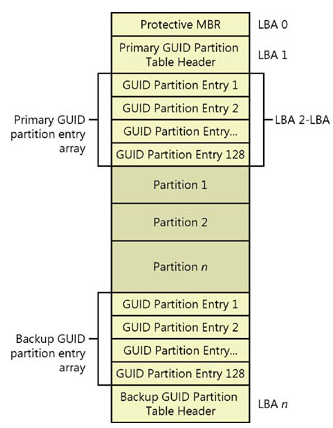
\includegraphics[width=0.46\textwidth]{images/gpt3.png}
 \end{center}
\end{frame}

\begin{frame}{File Systems - Particionado}
 \begin{itemize}
  \item Principales herramientas en Linux para particionar:
  \begin{itemize}
   \item parted 
   \item gparted
   \item fdisk
   \item gdisk
  \end{itemize}
  \vspace{0.2cm}
  \item Se usará parted porque soporta tanto MBR como GPT
 \end{itemize}
\end{frame}

\section{RAID}

\begin{frame}{RAID - Introducción}
  \begin{itemize}
   \item Problemas:
   \vspace{0.1cm}
   \begin{itemize}
    \item ¿Qué pasa si se rompe un disco? ¿Hay backup?
    \vspace{0.1cm}
    \item Si se llena un disco, ¿compro un disco más grande?
    \vspace{0.1cm}
    \item Velocidad de acceso. Operaciones I/O muy lentas
   \end{itemize}
   \vspace{0.2cm}
   \item Solución: 
   \begin{itemize}
    \vspace{0.1cm}
    \item RAID - Redundant Array of Independent Disks (originalmente llamado Redundant Array of Inexpensive Disks)
   \end{itemize}
 \end{itemize}
\end{frame}

\begin{frame}{RAID - Introducción (cont.)}
  \begin{itemize}
   \item RAID es una técnica que permite usar múltiples discos en forma conjunta con el fin de construir un sistema de discos 
      más rápido, más grande y más confiable
   \item Idea propuesta en 1988 en la Universidad de Berkley por los profesores David Patterson y Randy Katz y el 
      alumno Garth Gibson: ``A case for Redundant Arrays of Inexpensive Disks''
   \item Originalmente definía los niveles: 1,2,3,4,5
   \item En 1989, ``Disk System Architectures for High Performance Computing'' introdujo un nuevo nivel: RAID 6
   \item Ventajas sobre un solo disco (depende del nivel de RAID):
   \begin{itemize}
    \item Incremento de la perfomance
    \item Mayor capacidad
    \item Aumento de la confiabilidad
   \end{itemize}
  \end{itemize}
\end{frame}

\begin{frame}{RAID - Introducción (Cont.)}
  \begin{itemize}
   \item RAID provee las anteriores ventajas en forma transparente
   \item Para los file systems es un arreglo lineal de bloques que pueden ser leídos y escritos
   \item Internamente debe calcular que disco/s debe acceder para completar la solicitud
   \item Cantidad de accesos físicos de I/O depende del nivel de RAID que se está utilizando
   \item Diseñados para detectar y recuperarse de determinados fallos de discos
   \item {\bf Spare Disks:} discos disponibles para reemplazo de discos en falla  
  \end{itemize}
\end{frame}

\begin{frame}{RAID Level 0 - Striping}
 \begin{itemize}
  \item No es un nivel de RAID en absoluto. No existe redundancia. 
  \item Array de discos con “striping” a nivel de bloque
  \item Necesita 2 ó más discos para conformarse
  \item Capacidad del RAID: sumatoria de la capacidad de los discos participantes
  \item Sirve como ``upper-bound'' en cuanto a performance y capacidad  
  \item Si falla un disco, los datos de todos los disco se vuelven inaccesibles
  \item {\bf Stripe:} bloques en la misma línea 
 \end{itemize}
\end{frame} 

\begin{frame}{RAID Level 0 (cont.)}
 \begin{center}
  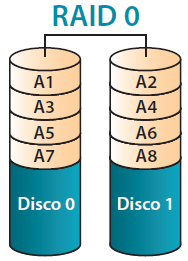
\includegraphics[width=0.4\textwidth]{images/raid0.png}
 \end{center}
\end{frame}

\begin{frame}{Chunk Size}
 \begin{center}
  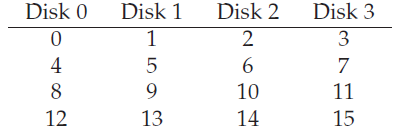
\includegraphics[width=0.6\textwidth]{images/chunk1.png}
 \end{center}
 \begin{center}
  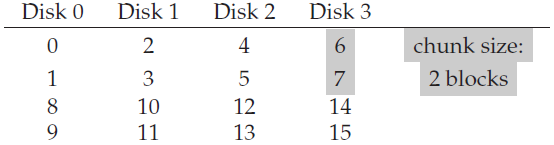
\includegraphics[width=0.65\textwidth]{images/chunk2.png}
 \end{center}
\end{frame}

\begin{frame}{RAID Level 1 - Mirroring}
 \begin{itemize}
  \item Asegura redundancia mediante el mirroring (espejado) de datos
  \item No hay striping de datos
  \item Almacena datos duplicados en discos separados o independientes
  \item Mínimo de 2 discos. Trabaja con pares de discos
  \item Ineficiente por la escritura en espejo
  \item Desperdicio del 50\% de la capacidad total
 \end{itemize}
\end{frame}

\begin{frame}{RAID Level 1 (cont.)}
 \begin{center}
  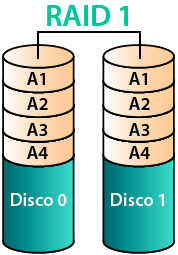
\includegraphics[width=0.4\textwidth]{images/raid1.png}
 \end{center}
\end{frame}

\begin{frame}{RAID Level 2}
 \begin{itemize}
  \item Striping a nivel de bit y paridad Hamming dedicada
  \item No muy aceptado por la industria
  \item Disco dedicados para almacenar información de verificación y corrección de errores
  \item Se requieren 3 discos como mínimo
  \item Buena protección de datos en caso de fallas de disco. Tasa de transferencia de datos puede llegar a ser muy elevada
 \end{itemize}
\end{frame}

\begin{frame}{RAID Level 2 (cont.)}
 \begin{center}
  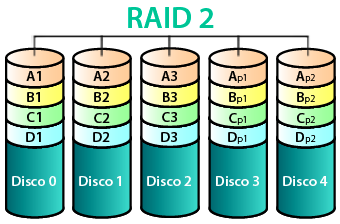
\includegraphics[width=0.6\textwidth]{images/raid2.png}
 \end{center}
\end{frame}

\begin{frame}{RAID Level 3}
 \begin{itemize}
  \item Striping a nivel de byte y paridad dedicada
  \item Disco “dedicado” para almacenar la información de paridad
  \item Datos se escriben en paralelo entre los disco del array
  \item 3 discos como mínimo
  \item Alta tasa de transferencia en escritura y lectura
  \item Disco de paridad puede convertirse en un cuello de botella  
  \item No ofrece solución al fallo simultáneo de disco
 \end{itemize}
\end{frame}

\begin{frame}{RAID Level 3 (cont.)}
 \begin{center}
  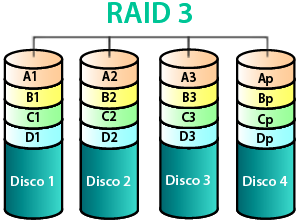
\includegraphics[width=0.6\textwidth]{images/raid3.png}
 \end{center}
\end{frame}

\begin{frame}{RAID Level 4}
 \begin{itemize}
  \item Striping a nivel de bloque y paridad dedicada
  \item 3 disco requeridos
  \item Alta tasa de transferencia de datos
  \item Controladora requerida es compleja, por lo tanto, costosa
 \end{itemize}
\end{frame}

\begin{frame}{RAID Level 4 (cont.)}
 \begin{center}
  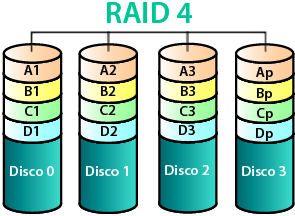
\includegraphics[width=0.6\textwidth]{images/raid4.png}
 \end{center}
\end{frame}

\begin{frame}{RAID Level 5}
 \begin{itemize}
  \item Striping a nivel de bloque y paridad distribuida
  \item Una de las implementaciones más utilizadas 
  \item Distribuye la información de paridad entre todos los discos del array
  \item 3 discos mínimo
  \item Alto rendimiento. No hay cuello de botella  
  \item No ofrece solución al fallo simultáneo de discos
 \end{itemize}
\end{frame}

\begin{frame}{RAID Level 5 (cont.)}
 \begin{center}
  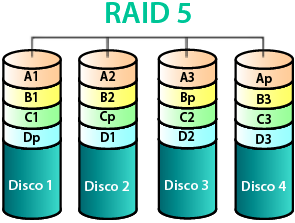
\includegraphics[width=0.6\textwidth]{images/raid5.png}
 \end{center}
\end{frame}

\begin{frame}{RAID Level 6}
 \begin{itemize}
  \item Striping a nivel de bloque y doble paridad distribuida
  \item Recomendado cuando se tienen varios discos
  \item Requiere 4 discos como mínimo
  \item Alta tolerancia a fallos (hasta dos discos)
  \item Operaciones de escrituras más lentas debido al calculo de la doble paridad
 \end{itemize}
\end{frame}

\begin{frame}{RAID Level 6 (cont.)}
 \begin{center}
  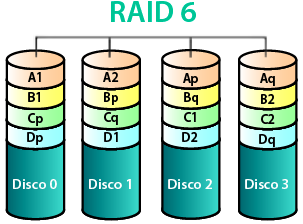
\includegraphics[width=0.6\textwidth]{images/raid6.png}
 \end{center}
\end{frame}

\begin{frame}{RAID - Niveles híbridos}
 \begin{itemize}
  \item Es posible combinar los distintos niveles de RAID
  \begin{itemize}
   \item RAID 0+1: Mirror of Striped Disks
   \item RAID 10(1+0): Stripe of Mirrored Disks
   \item RAID 50(5+0)
   \item RAID 100
   \item etc.
  \end{itemize}
 \end{itemize}
\end{frame}

\begin{frame}{RAID - Niveles híbridos - RAID 50}
 \begin{center}
  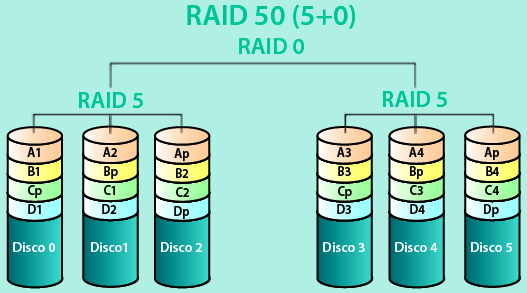
\includegraphics[width=0.7\textwidth]{images/raid50.png}
 \end{center}
\end{frame}

\begin{frame}{Configurar RAID Level 5}
 \begin{itemize}
  \item Particionar un disco. ¿Cuántas particiones necesarias cómo mínimo?
  \item Utilizar la herramienta parted para particionar el disco
 \end{itemize}
 \begin{center}
  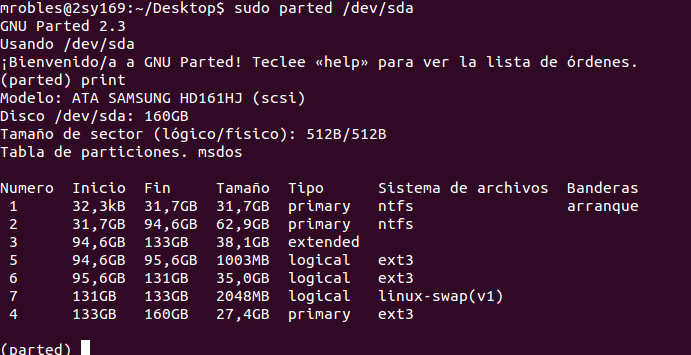
\includegraphics[width=0.6\textwidth]{images/partedmbr.png}
 \end{center}
\end{frame}

\section{LVM}

\begin{frame}{LVM - Introducción}
  \begin{itemize}
   \item ¿Qué tamaño le voy a dar a una partición?
   \item Logical Volume Management (LVM) provee un método más flexible que los convencionales esquemas
     de particionamiento para alocar espacio en los dispositivos de almacenamiento masivo 
   \item Escrito en 1998 por Heinz Mauelshagen (basó el diseño en el existente en HP-UX)
   \item Actualmente está en la versión 2
   \item Permite una administración ``on-line'' de los discos de almacenamiento agregando una capa adicional
     al subsistema de entrada del kernel
   \item Snapshots: backup on-line de las particiones  
  \end{itemize}
\end{frame}

\begin{frame}{LVM - Componentes}
 \begin{itemize}
  \item Principales componentes de LVM:
  \begin{itemize}
   \item {\bf Physical Volume (PV):} dispositivos físicos o particiones que serán utilizados por LVM
   \item {\bf Volume Group (VG):} grupo de PVs. Representa el ``data storage'' 
   \item {\bf Logical Volume (PV):} cada una de las partes en las que se dividen los VGs
   \item {\bf Physical Extent (PE):} unidades direccionables en las que LVM divide cada PV
   \item {\bf Logical Extent (LE):} unidad de alocación básica en los LVs
  \end{itemize} 
 \end{itemize}
\end{frame}

\begin{frame}{LVM - Componentes (cont.)}
 \begin{center}
  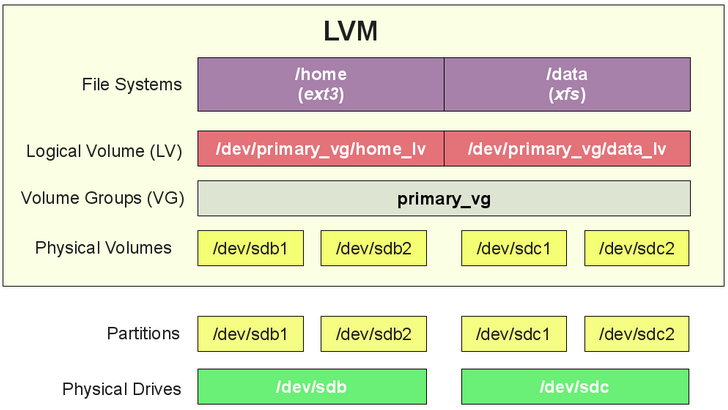
\includegraphics[width=0.8\textwidth]{images/lvm3.png}
 \end{center}
\end{frame}

\begin{frame}{LVM - Comandos}
  \begin{itemize}
   \item Generar 3 particiones (sean /dev/sda5, /dev/sda6 y /dev/sda7)
   \item Configurar estas particiones para que pueden trabajar por LVM
   \item {\it pvcreate /dev/sda5 /dev/sda6 /dev/sda7}  
   \item {\it pvscan} y {\it pvdisplay} para ver el estado de los PVs
  \end{itemize}
\end{frame}

\begin{frame}{LVM - Comandos}
  \begin{itemize}
   \item Siguiente paso: generar un VG en el PV creado en el paso anterior
   \item {\it vgcreate so\_test /dev/sda5 /dev/sda6 /dev/sda7}
   \item {\it vgscan} y {\it vgdisplay} para ver el estado de los PVs
   \item Es posible generar varios VG dentro de un PV
  \end{itemize}
\end{frame}

\begin{frame}{LVM - Comandos}
  \begin{itemize}
   \item Generar particiones lógicas en el VG generado en el paso anterior 
   \item Hay que indicarle el tamaño. Dos formas:
   \begin{itemize}
    \item {\it lvcreate -L 120G -n lv\_test so\_test }
    \item {\it lvcreate -l 25 -n lv\_test so\_test }  
   \end{itemize}
   \item {\it lvscan} y {\it lvdisplay} para ver el estado de los PVs
   \item Formatear el LV: {\it mkfs.ext3 /dev/so\_test/lv\_test}  
   \item Montar el LV en un punto de montaje 
  \end{itemize}
\end{frame}

\begin{frame}{LVM - Componentes (cont.)}
 \begin{center}
  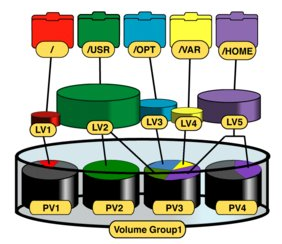
\includegraphics[width=0.7\textwidth]{images/lvm1.png}
 \end{center}
\end{frame}

\begin{frame}{Instalación Linux con Particionado Manual}
 \begin{itemize}
  \item Ubuntu Server 14.04
 \end{itemize} 
 \begin{center}
  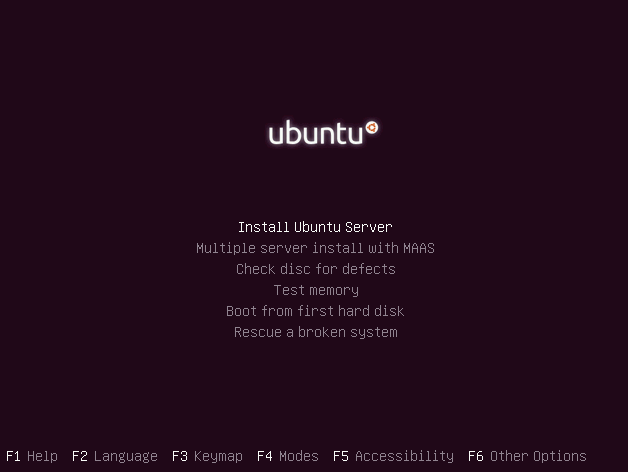
\includegraphics[width=0.7\textwidth]{images/install1.png}
 \end{center}
\end{frame}

\begin{frame}{Instalación Linux con Particionado Manual}
 \begin{center}
  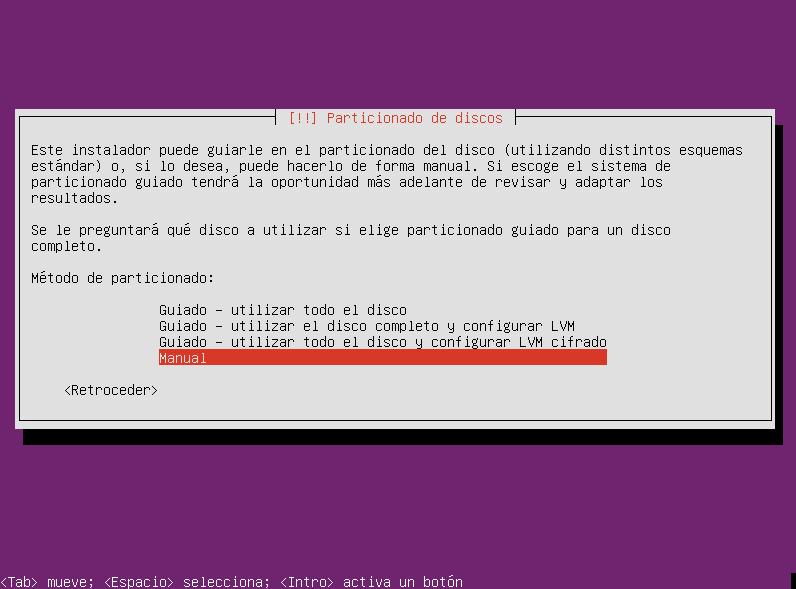
\includegraphics[width=0.8\textwidth]{images/install2.png}
 \end{center}
\end{frame}

\begin{frame}{Instalación Linux con Particionado Manual}
 \begin{center}
  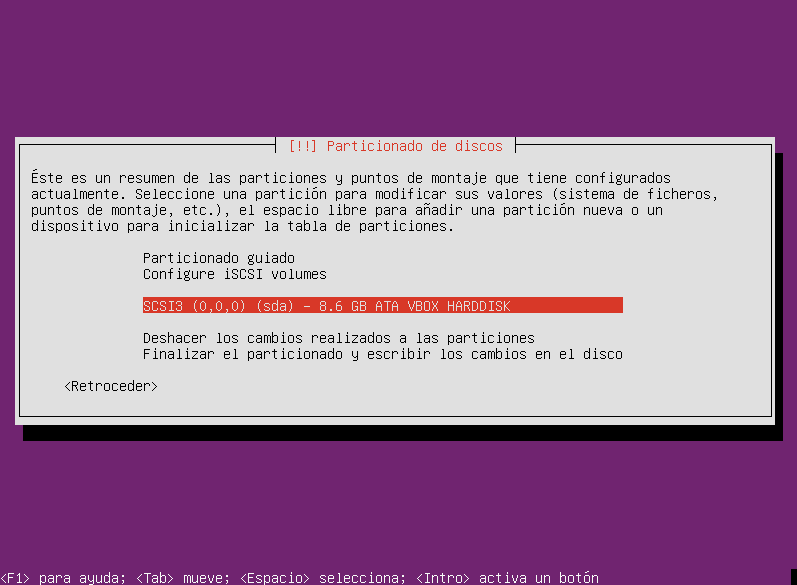
\includegraphics[width=0.8\textwidth]{images/install3.png}
 \end{center}
\end{frame}

\begin{frame}{Instalación Linux con Particionado Manual}
 \begin{center}
  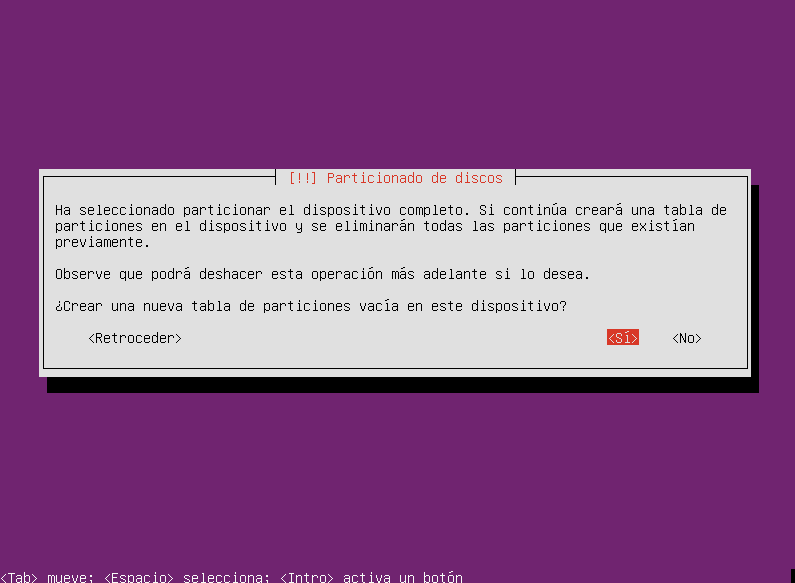
\includegraphics[width=0.8\textwidth]{images/install4.png}
 \end{center}
\end{frame}

\begin{frame}{Instalación Linux con Particionado Manual}
 \begin{center}
  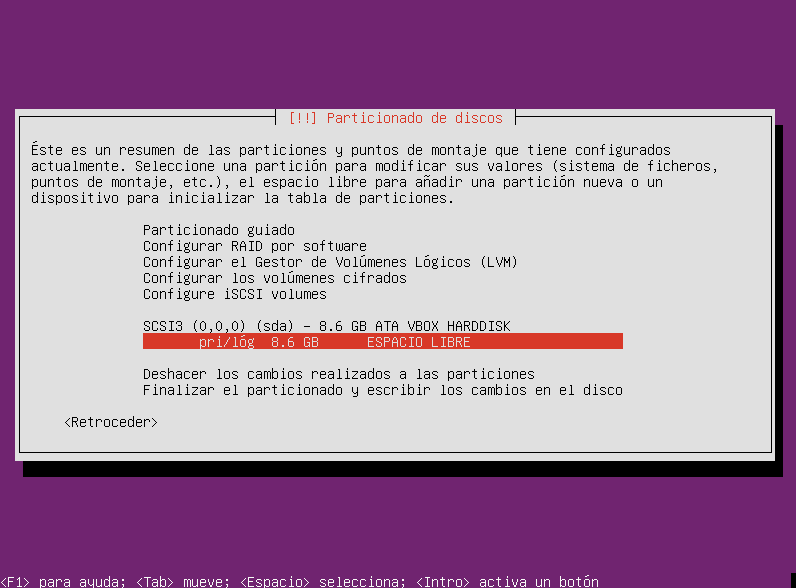
\includegraphics[width=0.8\textwidth]{images/install5.png}
 \end{center}
\end{frame}

\begin{frame}{Instalación Linux con Particionado Manual}
 \begin{center}
  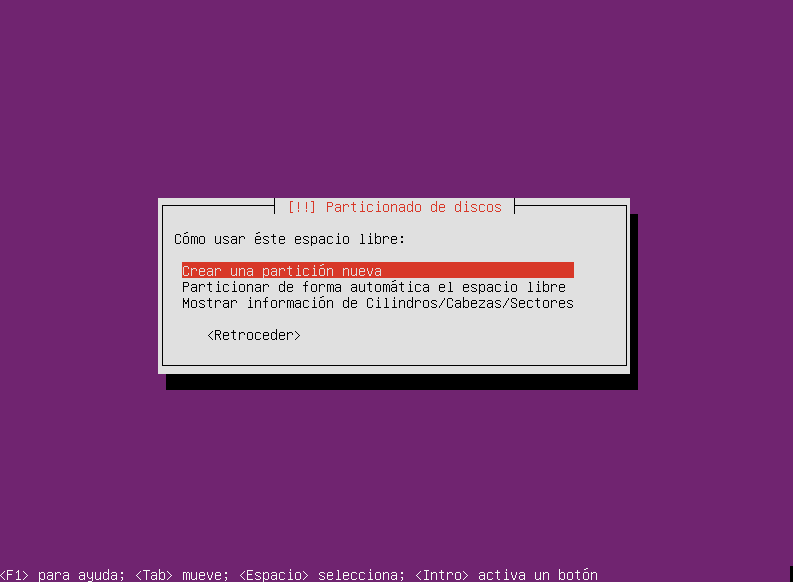
\includegraphics[width=0.8\textwidth]{images/install6.png}
 \end{center}
\end{frame}

\begin{frame}{Instalación Linux con Particionado Manual}
 \begin{center}
  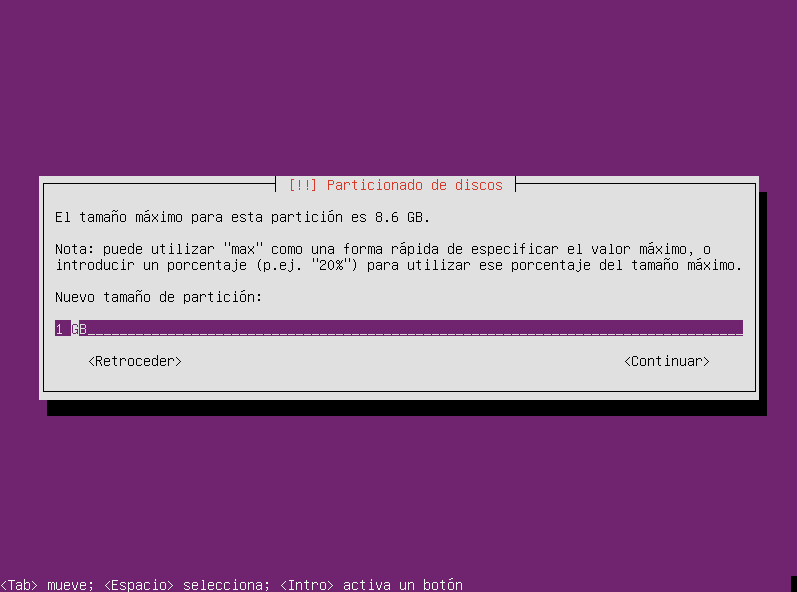
\includegraphics[width=0.8\textwidth]{images/install7.png}
 \end{center}
\end{frame}

\begin{frame}{Instalación Linux con Particionado Manual}
 \begin{center}
  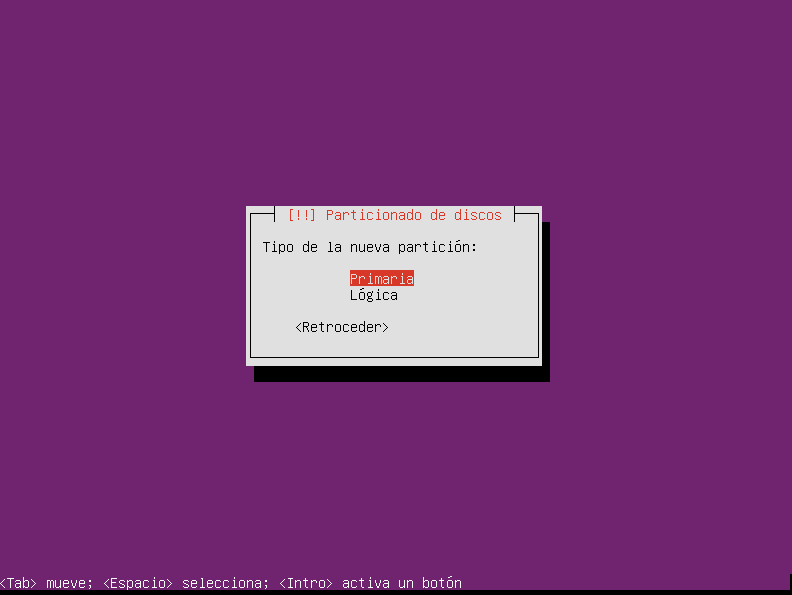
\includegraphics[width=0.8\textwidth]{images/install8.png}
 \end{center}
\end{frame}

\begin{frame}{Instalación Linux con Particionado Manual}
 \begin{center}
  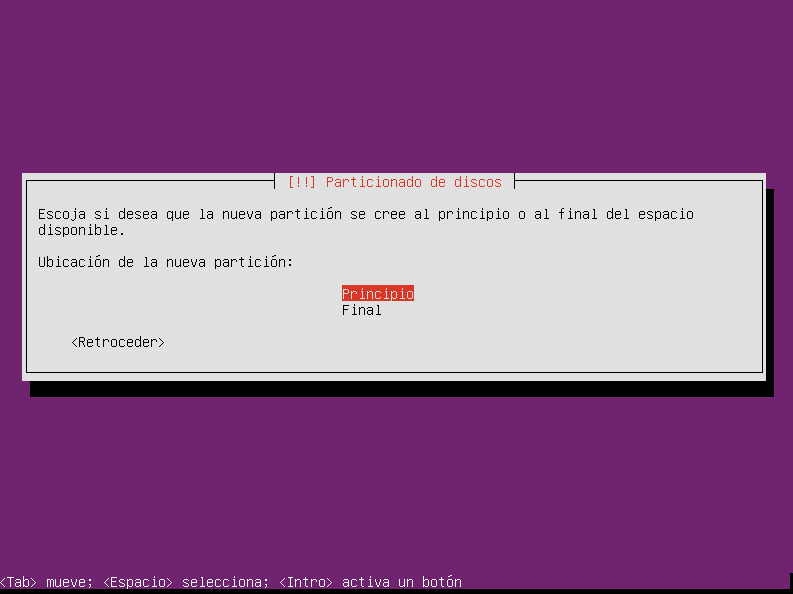
\includegraphics[width=0.8\textwidth]{images/install9.png}
 \end{center}
\end{frame}

\begin{frame}{Instalación Linux con Particionado Manual}
 \begin{center}
  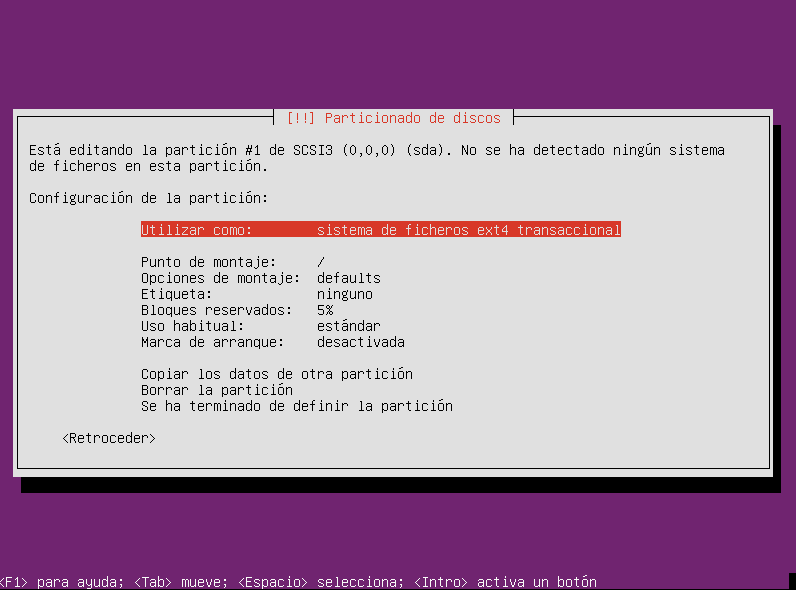
\includegraphics[width=0.8\textwidth]{images/install10.png}
 \end{center}
\end{frame}

\begin{frame}{Instalación Linux con Particionado Manual}
 \begin{center}
  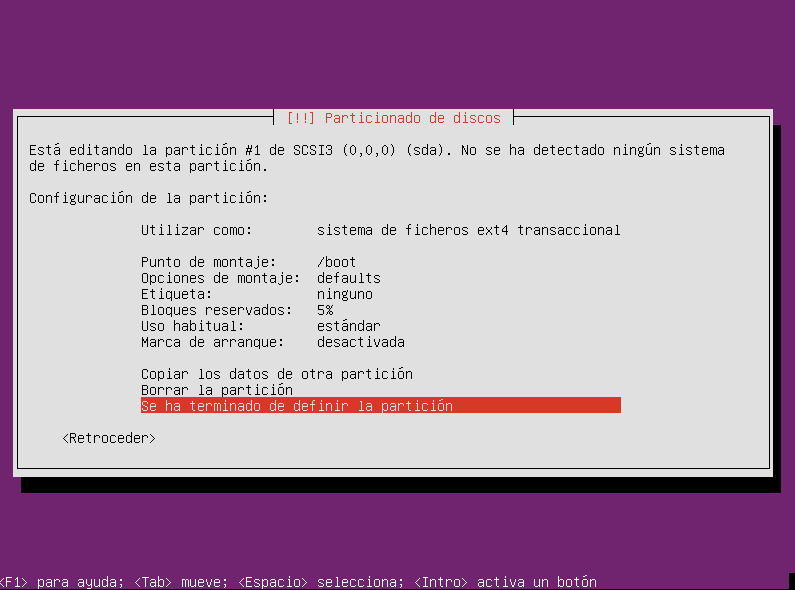
\includegraphics[width=0.8\textwidth]{images/install11.png}
 \end{center}
\end{frame}

\begin{frame}{Instalación Linux con Particionado Manual}
 \begin{center}
  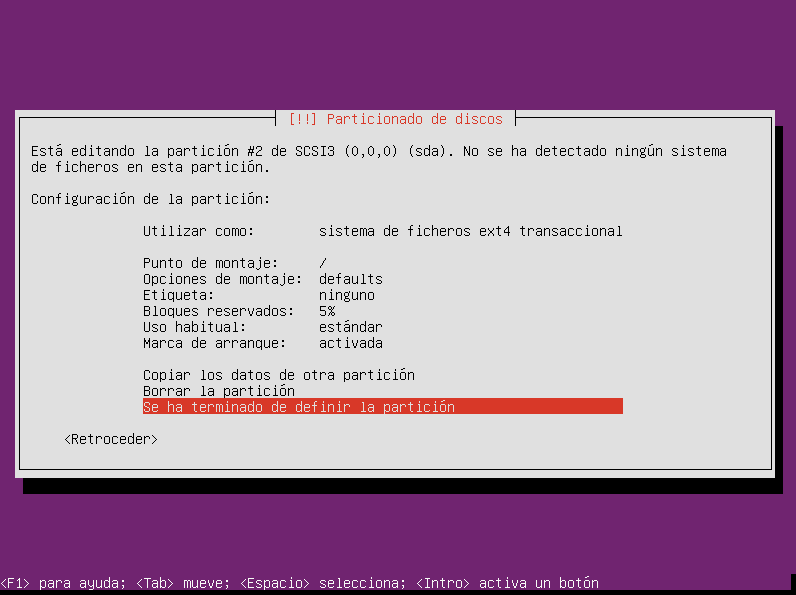
\includegraphics[width=0.8\textwidth]{images/install12.png}
 \end{center}
\end{frame}

\begin{frame}{Instalación Linux con Particionado Manual}
 \begin{center}
  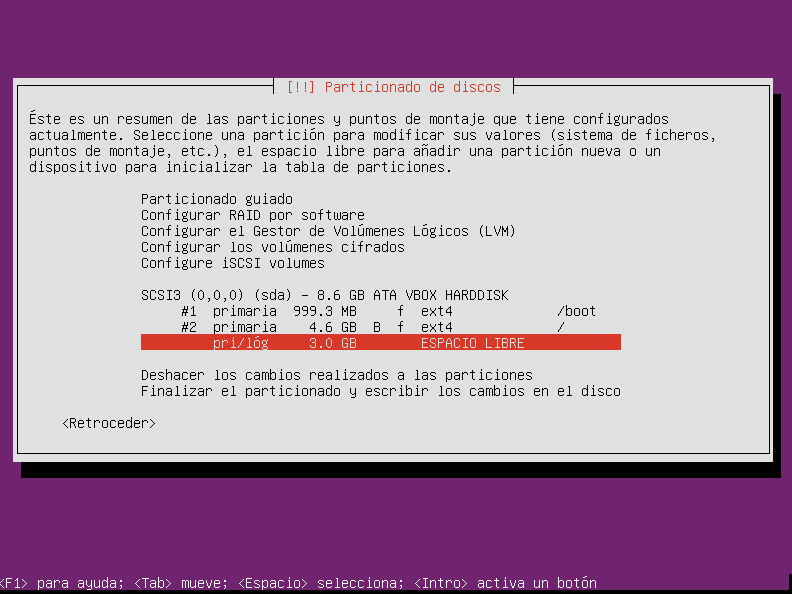
\includegraphics[width=0.8\textwidth]{images/install13.png}
 \end{center}
\end{frame}

\begin{frame}{Instalación Linux con Particionado Manual}
 \begin{center}
  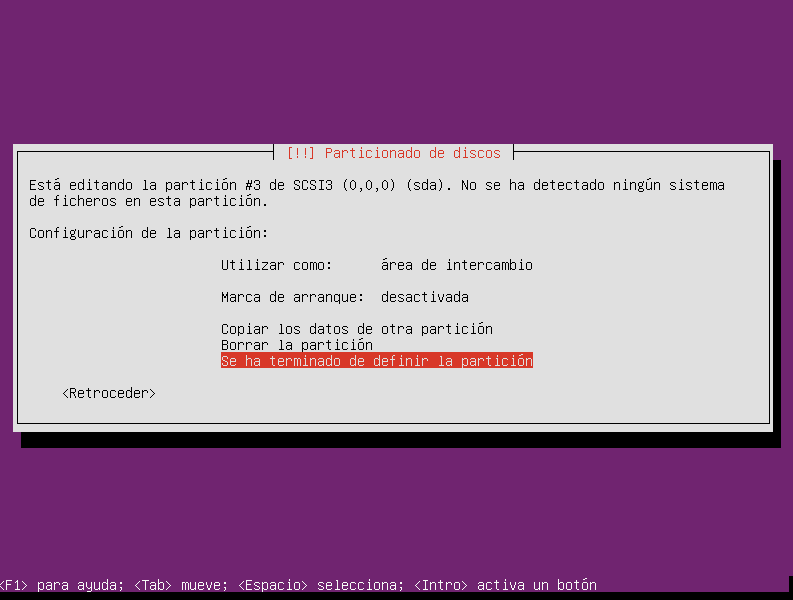
\includegraphics[width=0.8\textwidth]{images/install15.png}
 \end{center}
\end{frame}

\begin{frame}{Instalación Linux con Particionado Manual}
 \begin{center}
  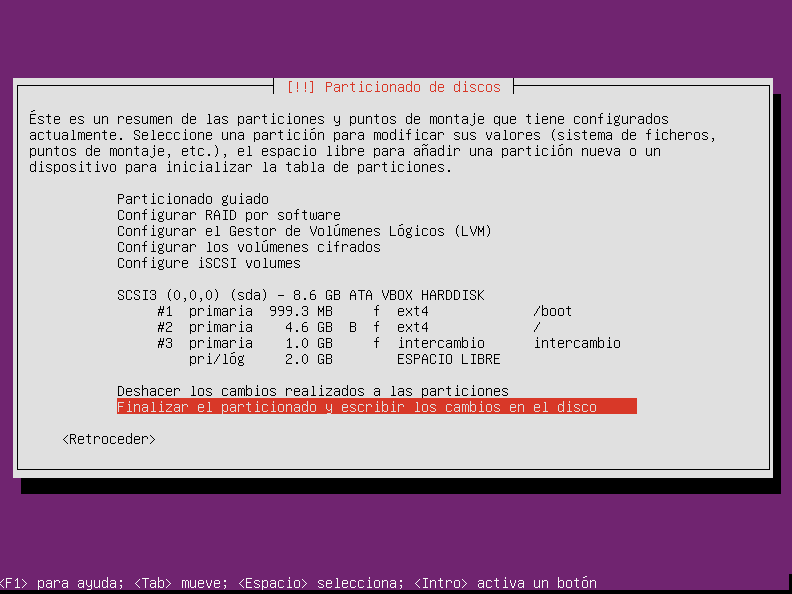
\includegraphics[width=0.8\textwidth]{images/install16.png}
 \end{center}
\end{frame}

\begin{frame}{Instalación Linux con Particionado Manual}
 \begin{center}
  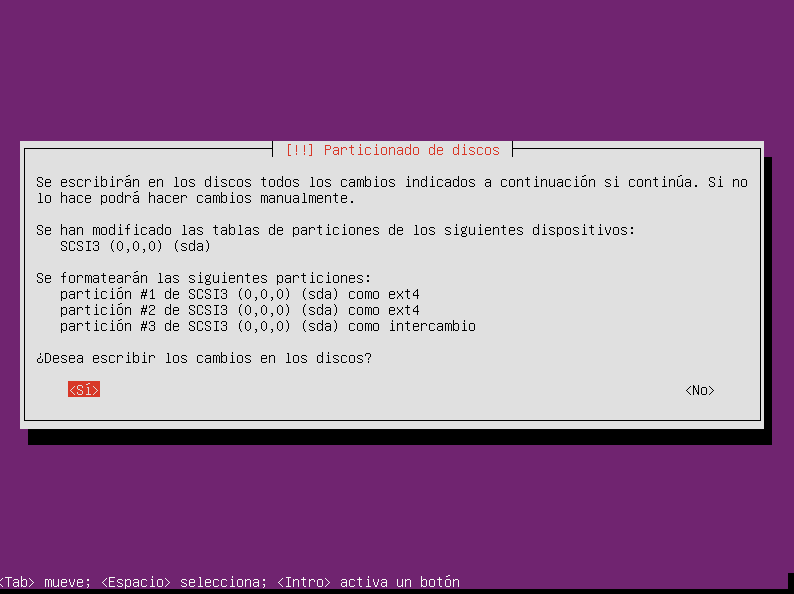
\includegraphics[width=0.8\textwidth]{images/install17.png}
 \end{center}
\end{frame}

\begin{frame}{Linux - Parted}
 \begin{center}
  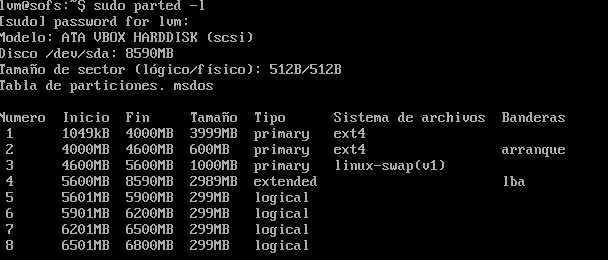
\includegraphics[width=0.8\textwidth]{images/parted5.png}
 \end{center}
\end{frame}

\end{document}

